%! TEX TS-program = xelatex
%! TEX encoding = UTF-8 Unicode

\documentclass{article}
\usepackage{fontspec, graphicx}
\usepackage{hyperref}
\usepackage{mathtools}
\usepackage[a4paper, margin=1in]{geometry}

\graphicspath{ {images/}}

\setmainfont{DejaVuSansMono}



\begin{document}
	\title{COMP3204 - Computer Vision\\Notes}
	\author{Bradley Mason\\ University of Southampton}
	\maketitle
	\newpage
	
	\tableofcontents
	\newpage
	\section*{Building Machines That See}
	\pagestyle{headings}
	\markright{L1 - Building Machines That See\hfill 01/11/16 \hfill}
	\addcontentsline{toc}{section}{L1 - Building Machines That See}
	A CCD is better than CMOS for sensitivity and noise.
	
	\newpage
	\section*{Local Features and Matching}
	\pagestyle{headings}
	\markright{L7 - Local Features and Matching \hfill 15/11/16 \hfill}
	\addcontentsline{toc}{section}{L7 - Local Features and Matching}
	\subsection*{Local Features and Matching Basics}
	Local feature points are used for:
	\begin{itemize}
		\item Image alignment
		\item Camera pose estimation and camera calibration
		\item 3D reconstruction
		\item Motion tracking
		\item Object recognition
		\item Indexing and database retrieval
		\item Robot navigation
	\end{itemize}
	A good example is panoramas, we need to {\bfseries match} and {\bfseries align} the images. You detect feature points in both images, find the corresponding pairs and then use those pairs to align the images.\\
	We can use two distinct types of matching problem.\\
	\\
	In stereo vision (vision with two cameras for 3D reconstruction) there are two important concepts related to matching:
	\begin{itemize}
		\item Narrow-baseline stereo
		\item Wide-baseline stereo
	\end{itemize}
	In {\bfseries Narrow Baseline Stereo} you have two images very close together. Similar to how human vision works. This is applicable to tracking where the object doesn't move too much between frames.\\
	In {\bfseries Wide Baseline Stereo} you have two images that are far apart and likely at completely different angles too. This is applicable to generic matching tasks like object recognition.
	
	\subsection*{Robust Local Description}
	The requirements of a descriptor are very much dependent on the task at hand.\\
	A narrow baseline is for when you need robustness to rotation and lighting is not so important. The descriptiveness can be reduced as search is over a smaller area.\\
	A wide baseline is for when you need robustness to intensity change and invariance to rotation. You have to be highly descriptive to avoid mismatches but not so distinctive that you can't find any matches. It is also robust to small localisation errors of the interest point, the descriptor shouldn't change too much if we move by a few pixels but to change rapidly once we move further away.
	
	\subsection*{Matching by Correlation}
	A.K.A Template Matching.\\
	For narrow baseline you may want to find the same point in two images that has shifted slightly. It can search the local area to match the template against the second image.\\
	Wide baselines are more tricky because they are not robust to rotation and you can't assume there will be a definable search area so you have to consider the entire second image which is likely to mismatch.
	
	\subsection*{Local Intensity Histograms}
	You can describe the region around an interest point with a pixel histogram. You can then measure the euclidean distance between these histograms to find the matching interest point.\\
	The problems with this is that it isn't very distinctive (remember the space image shuffled histogram being the same). It is also not rotation invariant if the sampling window is square or rectangular, which can be overcome with a circular window.\\
	It is also not invariant to illumination changes and sensitive to interest point localisation.\\
	You can overcome the localisation sensitivity by applying a weighting so pixels near the edge of the sample area have less effect than those near the interest point. It is very common to use Gaussian weighting centred on the interest point for the weighting.\\
	It is possible to make it illumination invariant by normalising or equalising the pixel patches before constructing the histogram or by using {\bfseries Local Gradient Histograms}
	
	\subsection*{Local Gradient Histograms}
	If you find the partial derivative of an image you can then compute the gradient orientations/directions and magnitudes.\\
	\\
	\begin{math}
	\theta = atan2(\frac{\delta f}{\delta y},\frac{\delta f}{\delta x}) \hspace{1cm}
	m = \sqrt{(\frac{\delta f}{\delta x})^2 + (\frac{\delta f}{\delta y})^2}
	\end{math}
	\\
	\\
	Instead of building histograms of the raw pixels values we can build histograms that encode the gradient magnitude and direction for each pixel in a sampling patch.\\
	Gradient magnitudes and directions are {\bfseries invariant to brightness} change!\\
	The gradient magnitude and direction histogram is also {\bfseries more distinctive}.\\
	\\
	In order to build these histograms you quantise the directions (0-360) into a number of bins (usually 8). Then for each pixel in the sampling patch you accumulate the gradient magnitude of that pixel in the respective orientation bin.\\
	\\By default this is not rotation invarient however it can be by finding the dominant orientation and cyclically shifting the histogram so the dominant orientation is the first bin.
	
	\subsection*{The SIFT Feature}
	{\bfseries SIFT} - Scale Invariant Feature Transform is very widely used.\\
	It builds on the idea of a logical histogram by incorporating {\bfseries spatial binning}, which in essence creates multiple gradient histogrms about the interest point and appends them into a longer feature.\\
	Standard SHIFT appends a spatial 4x4 grid of histograms with 8 orientations. This creates a 128 dimension feature which is both highly {\bfseries discriminative} and {\bfseries robust}!\\
	\\To construct this you find your interest point and take a sampling patch (commonly proportional to the scale of interest point). You then apply a Gaussian weighting centred around the interest point, this effectively reduces the corner to a 0 weighting changing this to a circular sample.\\
	You then take your 4x4 spatial bins and produce a gradient histogram for each using the gaussian weighting. The orientation is measured relative to the overall dominant orientation of the patch.
	
	\subsection*{Matching SIFT Features}
	The simplest way is to find the Euclidean distance and find the most similar in the second image. You can use a threshold to reject poor matches but unfortunately this also gives a lot of mismatches.\\
	It is better to take each feature and find the the two closest matches from the second images, only accept the first closest if the ratio between the two top matches is less than some threshold (typically 0.8 works best).\\
	This makes it much more robust.
	
	\newpage
	\section*{Image Search and Bags of Visual Words}
	\pagestyle{headings}
	\markright{L9 - Image Search and Bags of Visual Words \hfill 17/11/16 \hfill}
	\addcontentsline{toc}{section}{L9 - Image Search and Bags of Visual Words}
	
	\subsection*{Text Information Retrieval}
	A {\bfseries bag} is an {\bfseries unordered} data structure similar to a set. The main difference is that it allows elements to be inserted multiple times.\\
	A.k.a Multiset or counted set\\
	\\The processing of the text (feature extraction) then uses the following structure:\\
	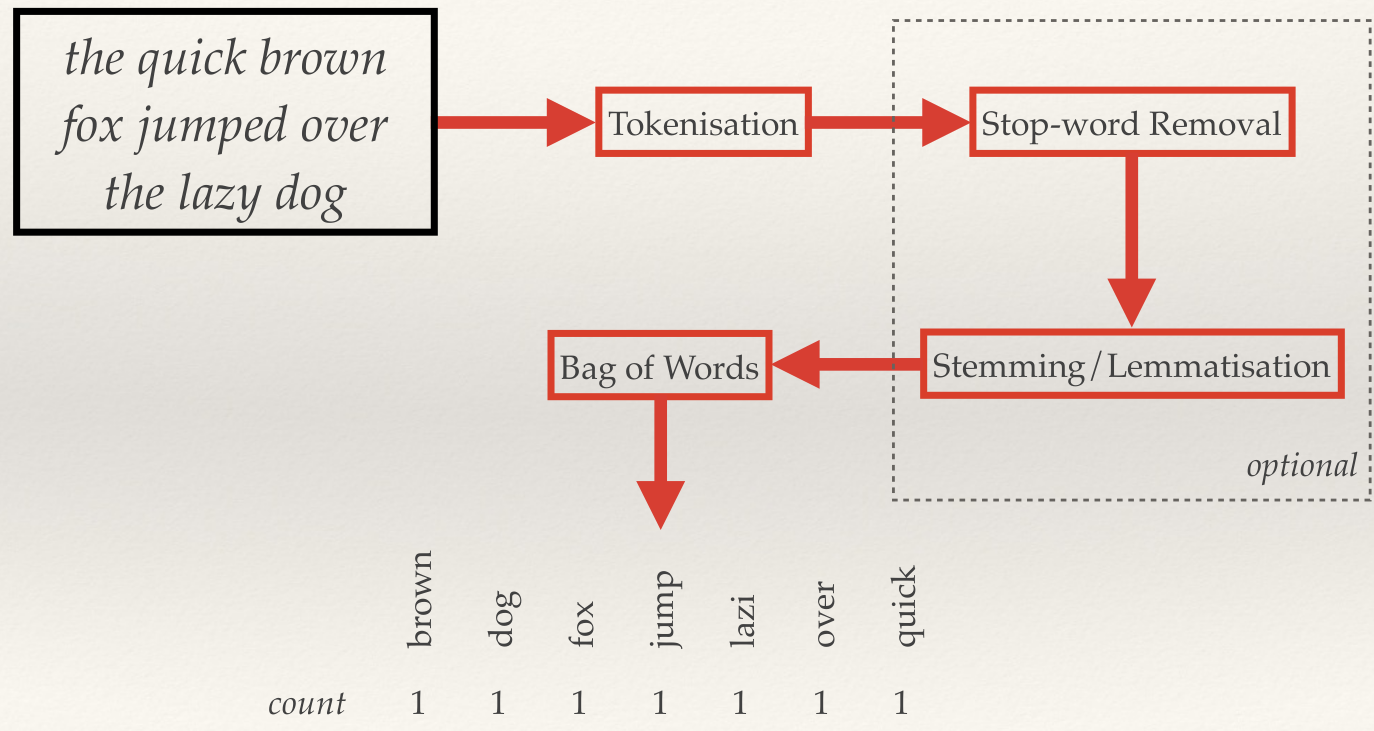
\includegraphics[scale=0.33]{text_processing}
	The {\bfseries Vector-Space Model} is conceptually simple.You model each document by a vector, and each query by a vector. You assume that documents close together in space are similar in meaning. You then uses standard similarity measures to rank each document to a query in terms of decreasing similarity.\\
	\\The {\bfseries lexicon} or {\bfseries vocabulary} is the set of all (processed) words across all documents known to the system.\\
	We can create vectors for each document with as many dimensions as there are words in the lexicon. Each word in the document's baf of words contributes a count to the corresponding element of the vector for that word. In essence, each vector is a histogram of the word occurences in the respective document. Vectors will have very high number of dimensions but will be very {\bfseries sparse}.\\
	If you took a graph with the word star on one axis and the word diet on the other, you could assume that a document with lots of "star" but little or no "diet" could be about astronomy. The converse might be about mammal behaviour whereas an equal high mixture of the two could be about a movie star.\\
	Here in the slides he does a recap of using cosine similarity to measure the distance between to words in a document, he speaks about how if we were to take into account every 0 value we would mainly be calculating 0 values with is inefficient. This suggests we should skip any 0 values words.\\Below is an example of the inverted index we might produce when measuring the words used in documents:\\
	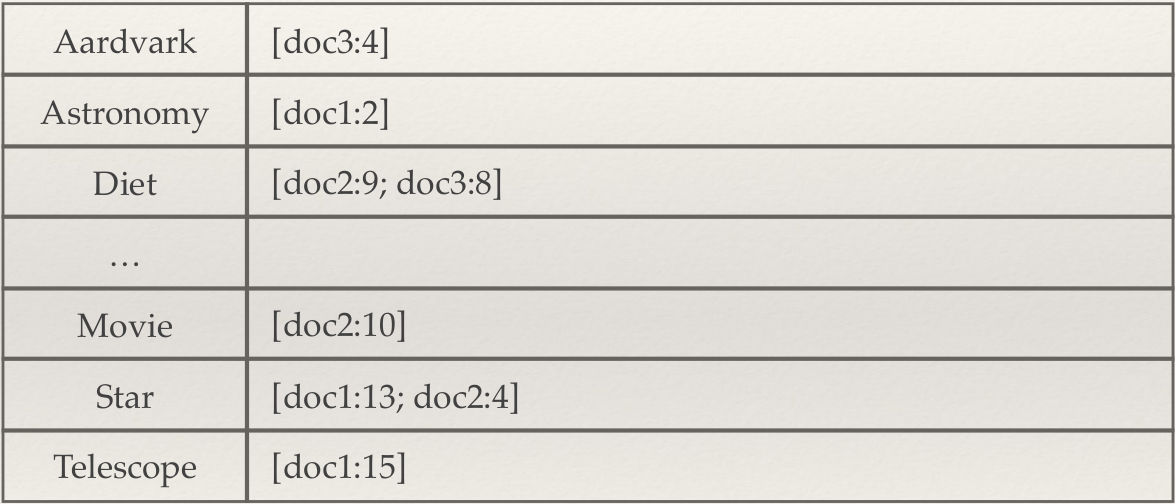
\includegraphics[scale=0.38]{inverted_index}
	It is much more efficient to calculate the cosine similarity by looking up the relevant postings list and accumulating similarities for only the documents seen in those postings list.
	The image below shows the accumulation table for the query "Movie Star". The multiplication is the number of times the word appear in the document x the number of times the word appears in the query. For instance, 10x1 is 10 times "Movie" from doc2 and 1 from query then 4x1 is 4 times "Star" from doc2.\\
	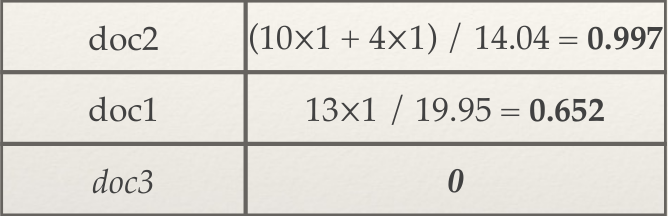
\includegraphics[scale=0.38]{accumulation_table}\\
	\\The number of times a word occurs in a document reflects the importance of that word in the document. A term that appears in many documents is not important as it can't distinguish them however if a term is frequent in a single document but rare elsewhere it is probably important in that document.\\
	Three possible weighting scemes are:\\{\bfseries Binary Weights} - Weight 1 or 0 dependin on whether it is present or not.\\
	{\bfseries Raw Frequency} - Frequemcy of term in a document is included in the vector.\\
	{\bfseries TF-IDF} - Where TF is Term Frequency which is the count of a term in a document. IDF is Inverse Document Frequency which provides high values for rare words and low values for common words.
	
	\subsection*{Vector Quantisation}
	{\bfseries Vector Quantisation} is a lossy data compression technique. Given a set of vectors, a technique like K-Means clustering can be used to learn a fixed size set of representative vectors. The representatives are the mean vector of each cluster in k-means. The set of representation vectors is called a {\bfseries codebook}.\\
	The quantisation is achieved by representing a vector by another approximate vector, which is drawn from a pool of representative vectors. Each input vector is assigned to the closest vector from the pool.
	
	\subsection*{Visual Words}
	We can vector quantise SIFT descriptors. Each descriptor is replaced by a representative vector known as a {\bfseries visual word}. This is in essence a small image patch with a certain pattern of pixels. In many ways this process is analogous to stemming words. The codebook is the visual equivalent of a lexicon or vocabulary.\\
	Once we've quantised the local features into visual words they can be put into a {\bfseries Bag of Visual Words}. Which ignores where in the image the local features came from.\\
	With these tools we are then able to produce histograms of visual occurences. Which is a way to aggregate a variable number of local descriptors into a fixed length vector.\\
	We have to consider the size of the vocabulary though because too smal and the vectors will look the same and it won't be very descriptive but too big and the words might never appear across images (too distinctive).
	
	\subsection*{Conent-based Image Retrieval}
	With the visual word representation we can apply everything used for text retrieval and apply it to images.\\
	The inverted index will only give performance gain if the vectors are sparse. This implies a very large codebook to avoid mismatching in images. There might be > 1 million visual words for SIFT vectors.\\
	This sort of size is non-trivial! It's very big.
	
	\subsection*{Overall Process for Building a BoVW Retrieval System}
	\begin{itemize}
		\item Collect the corpus of images that to be indexed and made searchable
		\item Extract local features from each image
		\item Learn a large codebook from a sample of the features
		\item Vector quantise the features and build BoVW representations for each image
		\item Construct an inverted index with the BoVW representations
	\end{itemize}
	
	\newpage
	\section*{Image Classification and Auto-Annotation}
	\pagestyle{headings}
	\markright{L10 - Image Classification and Auto-Annotation\hfill 22/11/16 \hfill}
	\addcontentsline{toc}{section}{L10 - Image Classification and Auto-Annotation}
	In images you can have multilabel classification. In this context it is often called Automatic Annotation. It uses object detection and localisation to find the different objects in the image.
	
	\subsection*{Challenges in Computer Vision}
	Object recognition in natural scenes * \\
	There is also scene/activity classification. Where you determine what activity is occuring in the image, e.g. playing music or cycling.\\
	Automatic annotation takes features from the image to select words that are contained within the image. An example in the slides shows the difficulty with some odd interpretations of images. For example an image of a polar bear has the annotations jeep, pair, face, pepper and model.
	\subsection*{The Semantic Gap}
	This is the fundamental problem of computer vision.\\
	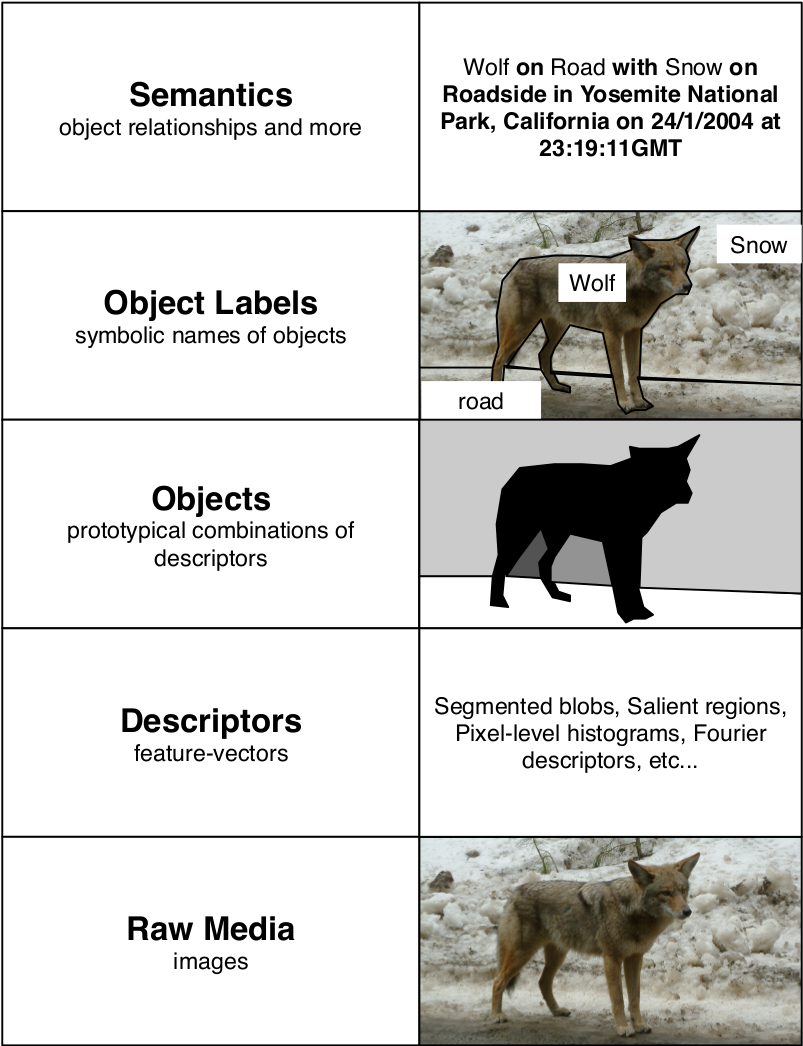
\includegraphics[scale=0.38]{semantic_gap}
	\subsection*{A Potted History}
	SIFT was discovered in 1999 and was very powerful but computationally demanding.\\
	Then in 2001 Cascades of Haar-like features was created, they were very popular for face detection.\\
	2006 introduced SURF matching had combined ideas from SIFT and the integral images used for computring Haar-like features.
	
\end{document}